\section{Hubo-Ach: Linux on Hubo}

\begin{figure*}[thpb]
  \centering
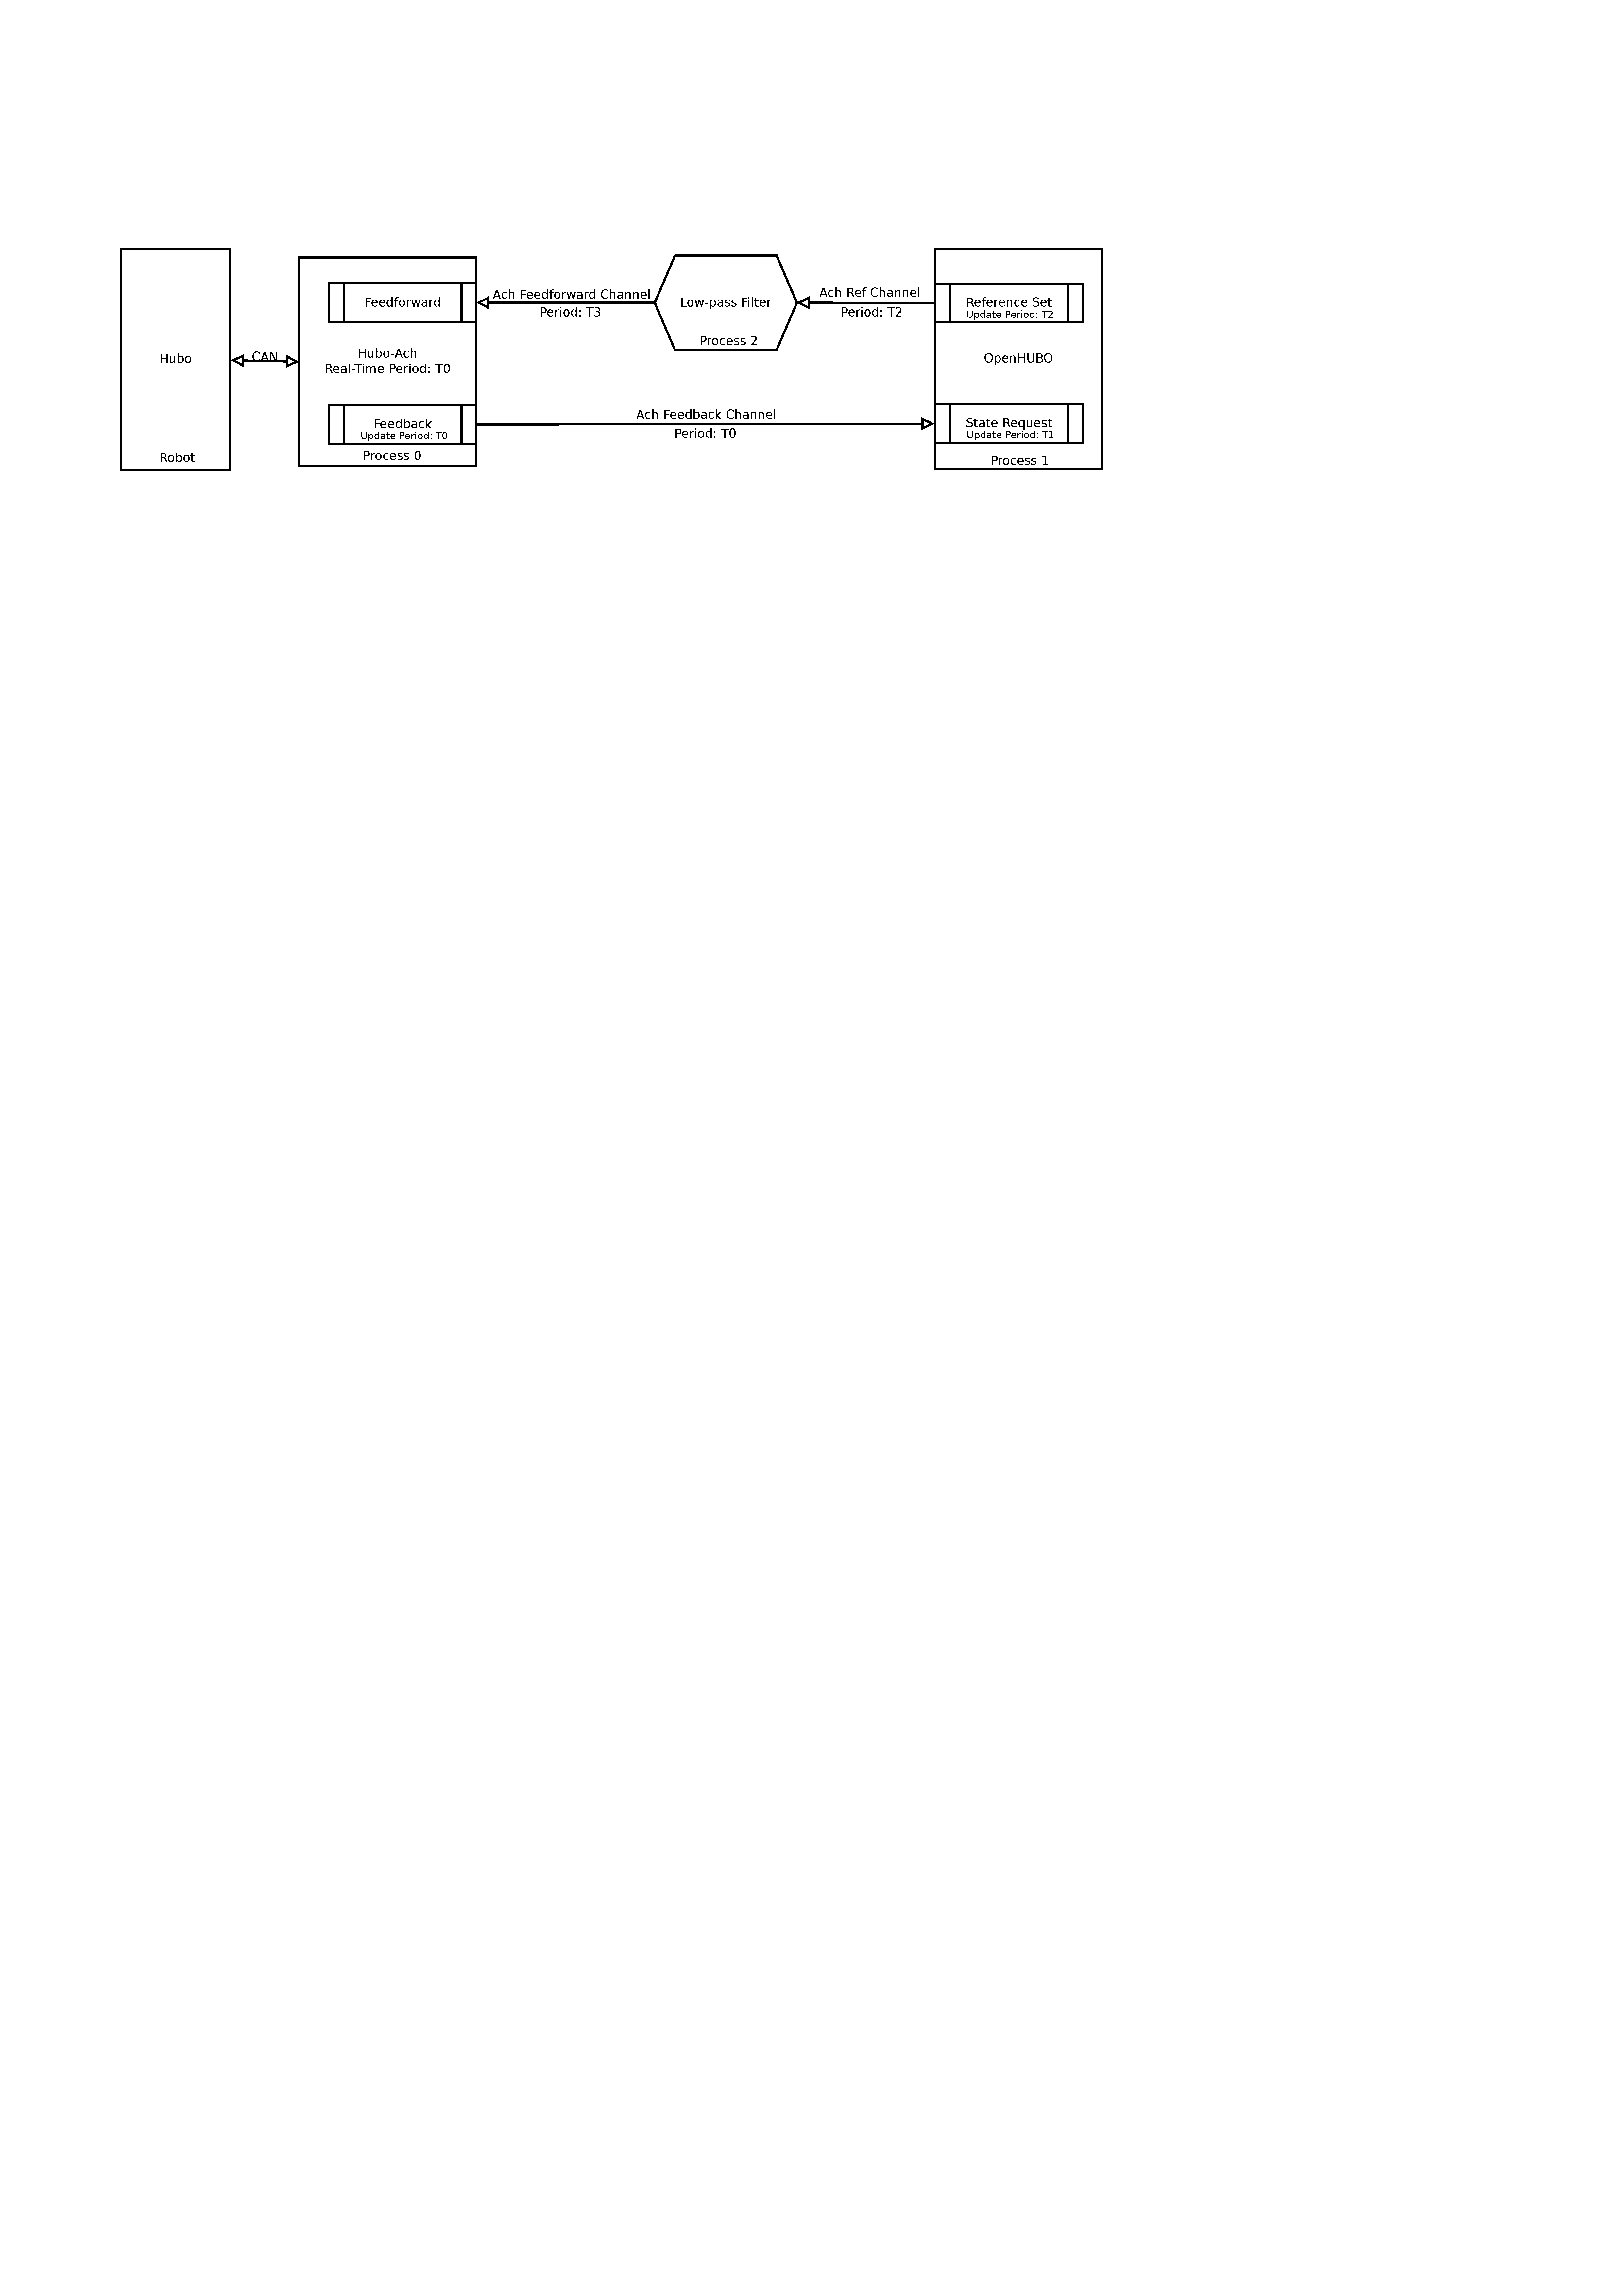
\includegraphics[width=2.0\columnwidth]{./pix/hubo-ach-diagram-OpenHUBO.pdf}
  \caption{Hubo-Ach interfacing with two seperate processes creating a closed loop system.  Process 0 (Hubo-Ach) takes the most recent command from the Feedforward Ach chanel and sends the reference command over the CAN bus to the Hubo.  The state date, including force-torque date from the ankles and wrists, IMU feed back, and actuial joint positions from the encoders are received and stored in the Feedback Ach chanel.  Process 1 (OpenHUBO) reads this data at its own rate, proforms the desired task such as calculating the inverse kinimatics inorder to pickup a cup and sends the the desired references to Process 2.  This process is a low-pass filter that reduces the jerk on each joint.  This smooths the desired trajectory allowing Process 1 to send step input to any of the joints. The reference command for each joint is set on the Feedforward Ach channel at a regular rate compleating the closed loop system.}
  \label{fig:graph}
\end{figure*}


Hubo now runs on the Linux based, open-source, BSD licensed, system called Hubo-Ach.  
Hubo-Ach is the brain child of Daniel M. Lofaro\footnote{Daniel M. Lofaro: http://danlofaro.com/} of DASL at Drexel University in collaboration with \textit{Golems - The Humanoid Robotics Laboratory}\footnote{Golems - The Humanoid Robotics Labatory: www.golems.org/} at the Georgia Institute of Technology.  

The overarching goal of the Hubo-Ach system is to create an easy to use interface between the Hubo hardware and the software environment.  
All system design decisions are made with the users, programmers and developers of the Hubo in mind.
This design philosophy streamlines closed-loop controller implementation, human robot interaction development and the utilization of popular robot related systems such as ROS\footnote{ROS: http://www.ros.org/} (Robot Operating System), OpenRAVE\footnote{OpenRAVE: http://openrave.org/} and MATLAB\footnote{MATLAB: http://www.mathworks.com/} on the Hubo platform.

Hubo-Ach is a single process that uses a high-speed, low-latency IPC called Ach \cite{ach} to comunicate with controllers that are indipendent processes.
Controllers are able to command each joint over an Ach channel at arbratary rates.
Hubo-Ach updates the motor references with the latest reference on the feedforward chanel at the rising edge of the real-time loop.
The real-time loop in Hubo-Ach is needed to ensure the internal phase lock loop (PLL) of the motor controller lock onto the reference update rate and to ensure the CAN bus bandwidth is not saturated.
This loop runs with a period of $T_0$.
$T_0$ is currently set to 0.005 $sec$.
This causes a CAN bus utiliztion of 78\%.

Fig.~\ref{fig:graph} shows how OpenHUBO (\textit{Process 1}) gets feedback from Hubo via the feedback Ach channel populated via Hubo-Ach.  
The OpenHUBO requests feedback data with a period of $T_1$.
If $T_1>T_0$ OpenHUBO will receive the most recent state data received by Hubo-Ach from the Hubo with no overlapping frames.
If $T_1<T_0$ OpenHUBO will receive the latest state data received by Hubo-Ach from the Hubo but some frames will overlap causing identical state data.
OpenHUBO performs calculations for tasks such as inverse kinimatcs for picking up cup, foot placement, etc.
Reference commands are created for each task and sent to \textit{Process 2} with a update period of $T_2$.
\textit{Process 2} is a low-pass filter that limits the jerk on each joint.
The resulting trajectory is sent to the Feedforward Ach chanel with a period of $T_3$.
$T_3$ is currently set to 0.01 $sec$.
This means that $T_2$ does not have to be a regular rate, it is possiable for $T_2>>T3$ and the commands sent to \textit{Process 2} can be a step input.
The resulting movements of Hubo are smooth and jitter free.





The key point is that Hubo-Ach updates the state data in the feedback Ach channel commands the motors with the references from the feedforward Ach channel in real-time with a preiod of $T_0$ no matter what rate the external controller is updating the feedforward channel.  









